\subsection{Grafical User Interface - GUI}
\label{subsec:GUI}

Die Bedienung der Kälteanlagen-SPS ist über zwei Wege möglich. Die erste Möglichkeit bietet TwinCat 3, indem sich der Benutzer auf die SPS \textit{einloggt} und die Codeausführen in Echtzeit nachvollziehen kann. Die Anlage lässt sich so steuern und überwachen. Es werden die Werte von Variablen- bzw. Symbolwerte angezeigt. Auf diese Art und Weise kann der SPS-Code debugged werden. 
Des Weiteren kann der Benutzer diese Bedienungart bei einer Fehlersuche, Testen von Programmen oder Parametereinstellungen einsetzen. 
Eine Fehlbedienung, z. B. durch \textit{Forcen} einer Variable auf einen Wert, kann unter Umständen zu Anlagenschäden führen. 

Die zweite Bedienmöglichkeit der SPS ist ein \textit{Grafical User Interface}(GUI). GUIs werden eingesetzt, um Prozessabläufe übersichtlicher darzustellen sowie Systemzustände schneller und effizienter interpretieren zu können. Die GUI wurde in Visual Studios in der Programmiersprache VB.NET erstellt. Grundlage für die GUI ist eine Instituts interne \textit{.DLL}-Bibliothek. Diese Bibliothek umfasst Benutzersteuerelemente wie beispielsweise Temperatursensoren, Dezimalanzeigen oder Sollwert-Eingaben. Für nähere Informationen über den informationstechnischen Aufbau der Bibliothek und der Steuerelemente wird auf die Arbeit von \citep{Nuerenberg2015} verwiesen. 
Neben der Institutsbibliothek kann auf die in Visual Studios vorhandenen Elemente wie Textboxen, Panels oder Timer zurückgegriffen werden. Diese Elemente werden von .NET Framework bereitgestellt.  

\subsubsection*{Uptown: RI-Fließbild}

\begin{figure}[htb]
\centering		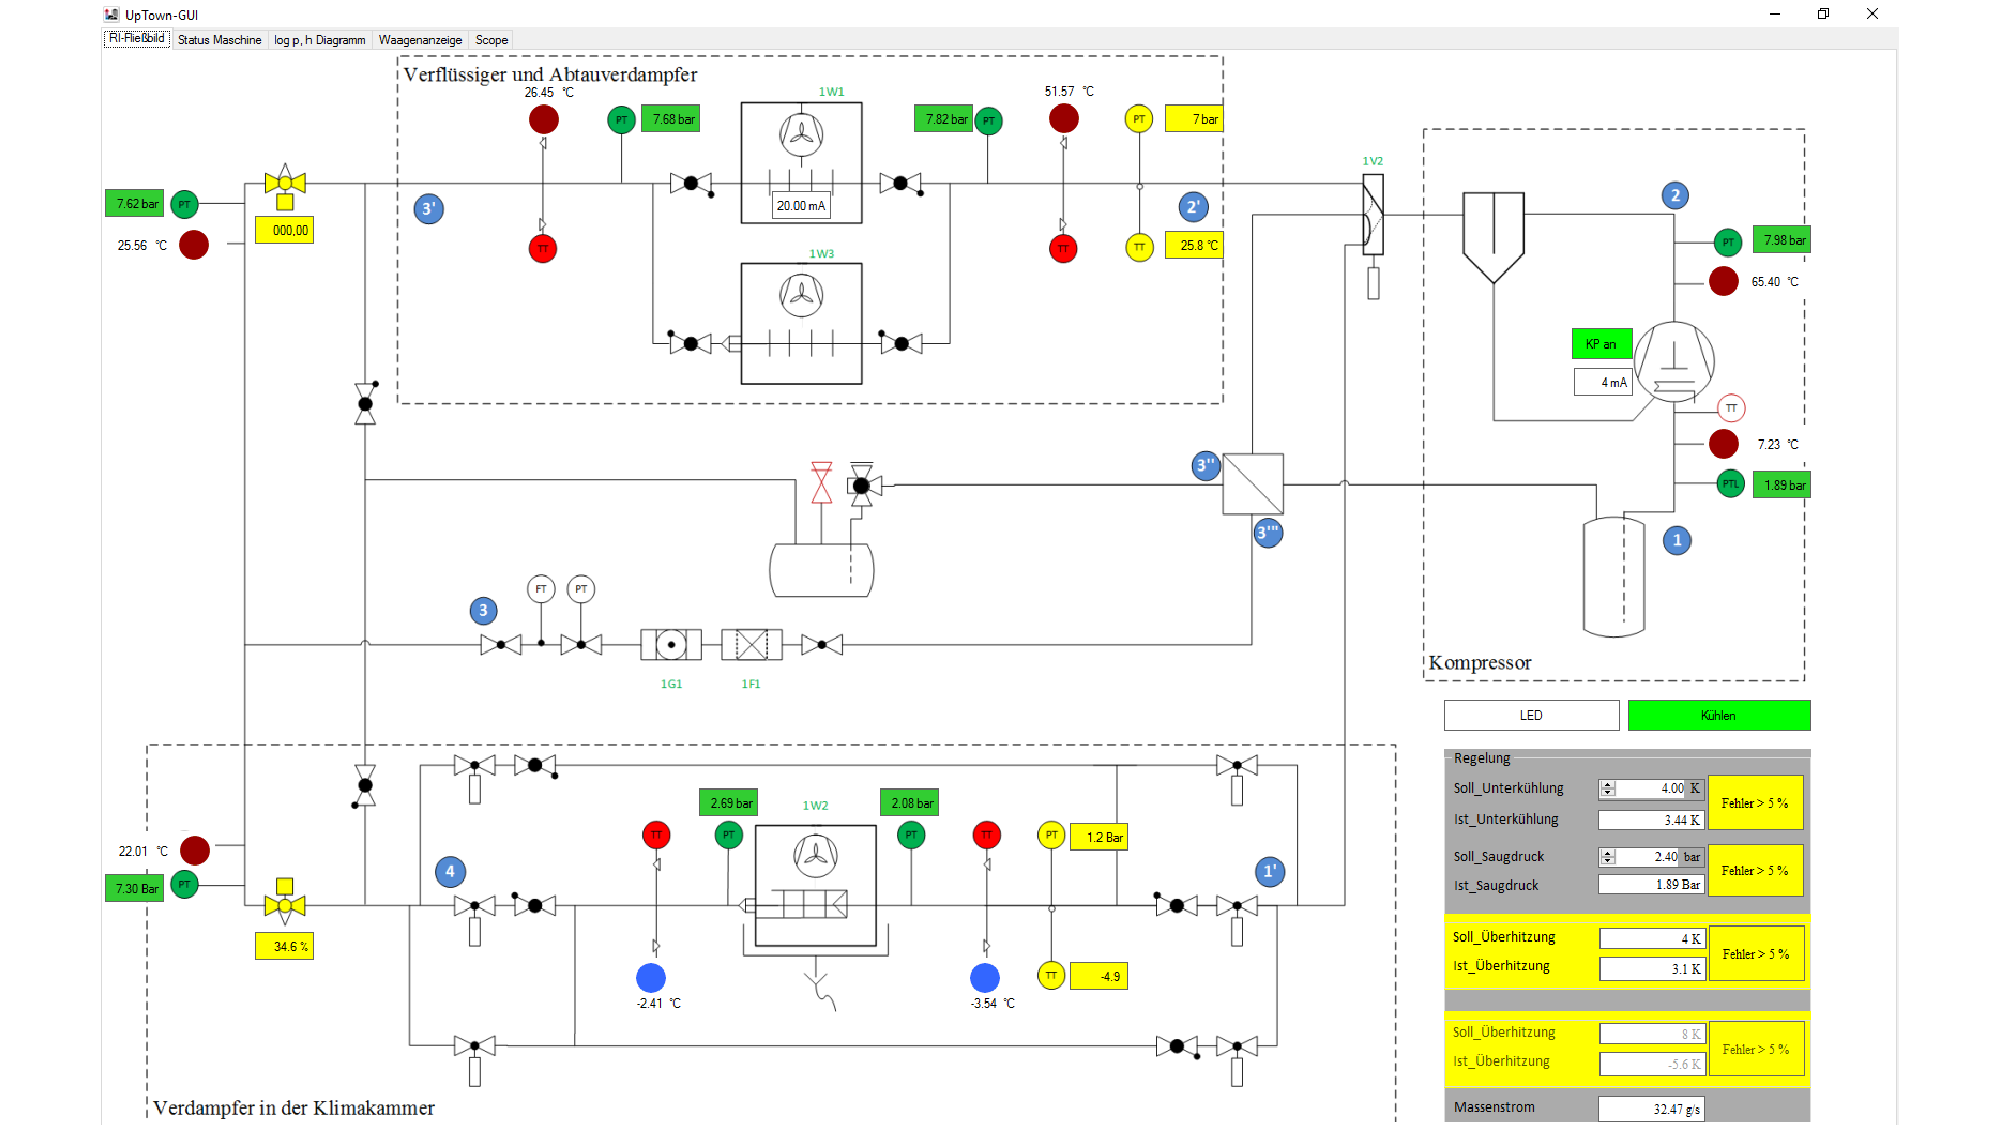
\includegraphics[page=1,width=1.05\textwidth]{Pictures/Versuchsaufbau/GUI.pdf}
\caption{RI-Fließbild in der GUI}
\label{fig:RI}
\end{figure}

Der erste Reiter der GUI ist das RI-Fließbild mit allen angeschlossenen Sensoren. Es gibt dem Benutzer einen Überblick über den Maschinenzustand der Anlage. Alle Temperatursensoren haben neben ihrer Dezimalanzeige einen roten, über 0 °C, bzw. blauen,unter 0 °C, Punkt. Die Drucksensoren sind alle grün dargestellt und die Expansionsventil-Sensoren jeweils in gelb. Neben dem Kompressor steht der aktuelle Steuerstrom. Ein LED rechts neben dem Kompressor gibt an, ob das Kompressor-Schütz an oder aus ist. 
Beim Verflüssiger wird ebenfalls der aktuelle Steuerstrom angezeigt. 

Unten rechts im Reiter stehen die Istwerte und die Sollwerte der PID-Regler. Die Sollwerte lassen sich verändern. Der Soll-Unterkühlungswert der Expansionsventile lassen sich nicht per SPS einstellen. Änderungen für einen Parameter in den Einstellungen oder Sollwert-Änderung, deswegen müssen jegliche Änderungen am Expansionsdisplay händisch durchgeführt werden. Ist der Fehler eines PID-Regler kleiner als 5 $\%$ Abweichung, so wird das LED grün.     


\subsubsection*{Uptown: Steuerung über Statusmaschine}

\begin{figure}[htb]
\centering		\includegraphics[page=2,width=1.05\textwidth]{Pictures/Versuchsaufbau/GUI.pdf}
\caption{RI-Fließbild-Reiter in der GUI}
\label{fig:RI}
\end{figure}

Auf der zweiten Seite der GUI ist die Steuerung abgebildet. Hier lässt sich die KA starten, steuern und ausschalten. Links in der grauen Box sind die Transitionsvariablen für die Bedienung der Statusmaschine angebracht. 

Die KA verfügt über einen \textit{Automatik-Modus}. Für den Automatikmodus muss eine Vereisungszeit und eine Abtaumethode ausgewählt werden. Die Statusmaschine führt dann die Transitionen zwischen Vereisung und Abtauen automatisch durch. Sind die zwei Parameter eingestellt, muss nur noch \textit{Kühlen} aktiviert werden und die Statusmaschine führt die Messungen automatisch durch. 

In dem blau hinterlegtem Feld beziehen sich auf den Kühlmodus; rot hinterlegt auf den Abtaumodus. Über \textit{Kühlen} wird der Vereisungsvorgang gestartet und über \textit{Kühlen abbrechen} wieder gestoppt. Wurde \textit{Kühlen} aktiviert, so startet die KA automatisch mit dem Modus \textit{Vollautomatik}. Der \textit{Manueller Modus} ist nur für besondere Zweck in der Inbetriebnahme zu verwenden.

Über \textit{Abtauen} lässt sich ein Abtaumodus starten. Ist \textit{Abtauen} aktiviert, kann die beliebige Abtaumethode ausgewählt werden. Erst nach Auswahl der Abtaumethode startet der Abtauvorgang (vgl. \ref{subsec:Statusmaschine}: Statusmaschine: Abtauen ). Soll der Abtauvorgang abgebrochen werden, so muss \textit{Abtauen abbrechen} aktiviert werden. Im Modus \textit{elektrisch Abtauen}, kann die Heizstufe geändert werden. Die Heizstufe muss zwischen 0 und 10 V liegen. Liegt sie außerhalb, so wird automatisch das obere oder untere Limit als Heizstufe gesetzt. Bei einer Heißgas-Abtauung kann zusätzlich die \textit{Abtauzeit} eingestellt werden. Die \textit{Abtauzeit} ist bestimmt die Dauer, die das Heißgas durch den vereisten Verdampfer strömt.  

Die zwei untersten Checkfelder sind \textit{PumpDown durchführen} und \textit{PumpDown$\_$rev durchführen}. Die zwei Vorgänge dienen der Kältemittelrückführung in den Sammler. Ein bis mehrere PumpDowns sollten vor dem Anlagenstillstand durchgeführt werden, um möglichst viel Kältemittel in den Sammler zu befördern. 

In der Mitte befindet sich die Ablaufstruktur der Statusmaschine. Das Bild dient nur der gesamte Übersicht über den Prozess und dan Ablauf. Im obereren rechten Teil sind die Komponenten des Kältekreislaufes aufgelistet. Die LEDs neben den Komponenten geben Auskunft darüber, ob die Komponenten an- oder ausgeschaltet sind.   Über das Schaltfeld \textit{SPS} wird die ADS-Verbindung zur SPS hergestellt. Bei "grün" ist eine Verbindung hergestellt und bei "rot" besteht keine Verbindung. 



\subsubsection*{Uptown: Log p,h-Diagramm}

\begin{figure}[htb]
\centering		\includegraphics[page=3,width=1.05\textwidth]{Pictures/Versuchsaufbau/GUI.pdf}
\caption{log p,h-Diagmramm-Reiter in der GUI}
\label{fig:RI}
\end{figure}

Der dritte Reiter der GUI ist eine Darstellung der Zustandspunkte in einem log p,h-Diagramm. Jeder Zustandspunkt ist in einem magenta farbigen Punkt inklusive seiner Bezeichnung in dem Diagramm wiederzufinden. Die Darstellung gibt dem Benutzer sehr schnell Auskunft über den Zustand des Systems. Jeder Zustandspunkt wird jede Sekunde aktualisiert. 

Zusätzlich sind die Zustandspunkt mit ihren zugehörigen Werten von Druck, Temperatur und Enthalpie im grauen Fenster hinterlegt. Für den Kompressor, Verflüssiger und den Verdampfer gibt die letzte Spalte den bilanzierten Wärmestrom jeder Komponente in kW an. 

\subsubsection*{Uptown: Wägesystem}

\begin{figure}[htb]
\centering		\includegraphics[page=4,width=1.05\textwidth]{Pictures/Versuchsaufbau/GUI.pdf}
\caption{Wägesystem-Reiter in der GUI}
\label{fig:RI}
\end{figure}

Der Reiter des Wägesystems ist aufgeteilt in 3 Bereiche (markiert mit 1,2,3). Der erste Bereich, links, stellt den Luftkühler aus einer Vogelperspektive dar. Das ermittelte Gewicht der eingesetzten Waagen ist in unterschiedlichen Farben hinterlegt und befinden sich unter den Aufhängepunkten des Luftkühlers auf den Blattfedern. Die farblich hinterlegte Anzeige zeigt die Gewichtsanzeige nach dem "TARE"-Befehl. Die in grau hinterlegte Anzeige zeigt das tatsächliche, gemessene Gewicht der Waage. 

Der mittlere Bereich(mit 2 makiert) zeigt den Luftkühler von der Seite. Hier sind 4 Oberflächentemperaturfühler am jeweils Eingang der Wärmeübertragerpacks. Der Verdampfer besteht aus vier solcher Wärmepacks. Neben den Oberflächentemperaturfühler sind auch noch der Ein- und Ausgang des Verdampfers mit einem Temperaturfühler versehen. Unter dem Luftkühler befindet sich die fünfte Waage, die das Schmelzwasser wiegt. 

Der rechte Bereich (markiert mit 3) ist aufgeteilt in weitere Zwei Reiter:
\begin{itemize}
\item	\textit{Anleitung Kalibrierung}
\item	\textit{Messwerte}.	
\end{itemize}


Der Karteireiter \textit{Messwerte} stellt verschiedene Messkurven dar. Die Messkurven entsprechen Messprojekten aus TwinCat und werden über ein Benutzerelement in die GUI integriert. Über die Bedienflächen lassen sich Messungen starten und stoppen und falls gewünscht auch als Scope-Datei exportieren. Zurzeit sind 4 Messkurven unter \textit{Messwerte} hinterlegt:

\begin{itemize}
\item	Waagen
\item	Bereifungsmenge
\item	2D-Schwerpunkt
\item 	Ventilöffnung vom Expansionsventil
\end{itemize}

In dem Reiter Waagen-Kalibrierung wird der Benutzer durch den Waagen-Kalibrierungsprozess geleitet. Dieser besteht aus (a)Gewichts-Kalibrierung, (b)Ventilator-Kalibrierung und (c)Reset-Waagen, siehe Abbildung \ref{fig:AnleitungKalibrierung}.  Der gesamte Kalibrierungsprozess dauert 1 h, weiter Informationen siehe Abschnitt \ref{sec:Kalibrierung Wägesystem}. 


\begin{figure}[htb]
\centering		\includegraphics[width=0.40\textwidth]{Pictures/GUI/AnleitungKalibrierung.png}
\caption{Karteireiter \textit{Anleitung Kalibrierung}}
\label{fig:AnleitungKalibrierung}
\end{figure}

\subsubsection*{Uptown: Scope}

\begin{figure}[htb]
\centering		\includegraphics[page=5,width=1.05\textwidth]{Pictures/Versuchsaufbau/GUI.pdf}
\caption{Scope-Reiter in der GUI}
\label{fig:RI}
\end{figure}

Unter dem Karteireiter \textit{Scope} sind alle Komponenten des Kältekreislaufes bilanziert. Für jede Komponente ist die Ein- und Ausgangstemperatur und -druck abgebildet. Für den Luftkühler sind zusätzlich noch die 4 Oberflächentemperaturen bei den Temperaturen integriert. Nach dem die Graphen gestartet worden sind, lassen sie sich jeder Zeit per \textit{Pausen}-Symbol anhalten und per Zoomfunktion genauer untersuchen. 
Aus Lizenzgründen lassen sich Prozesse maximal eine Stunde lang mit aufzeichnen. 
Unter "Datei$\rightarrow$ Datei laden " lassen sich beliebige Scope-Measurementprojekte in den Karteireiter laden und ausführen. 